\documentclass[tikz,border=8pt]{standalone}
\usepackage[utf8]{inputenc}
\usetikzlibrary{arrows.meta,positioning,shapes.geometric}
\begin{document}
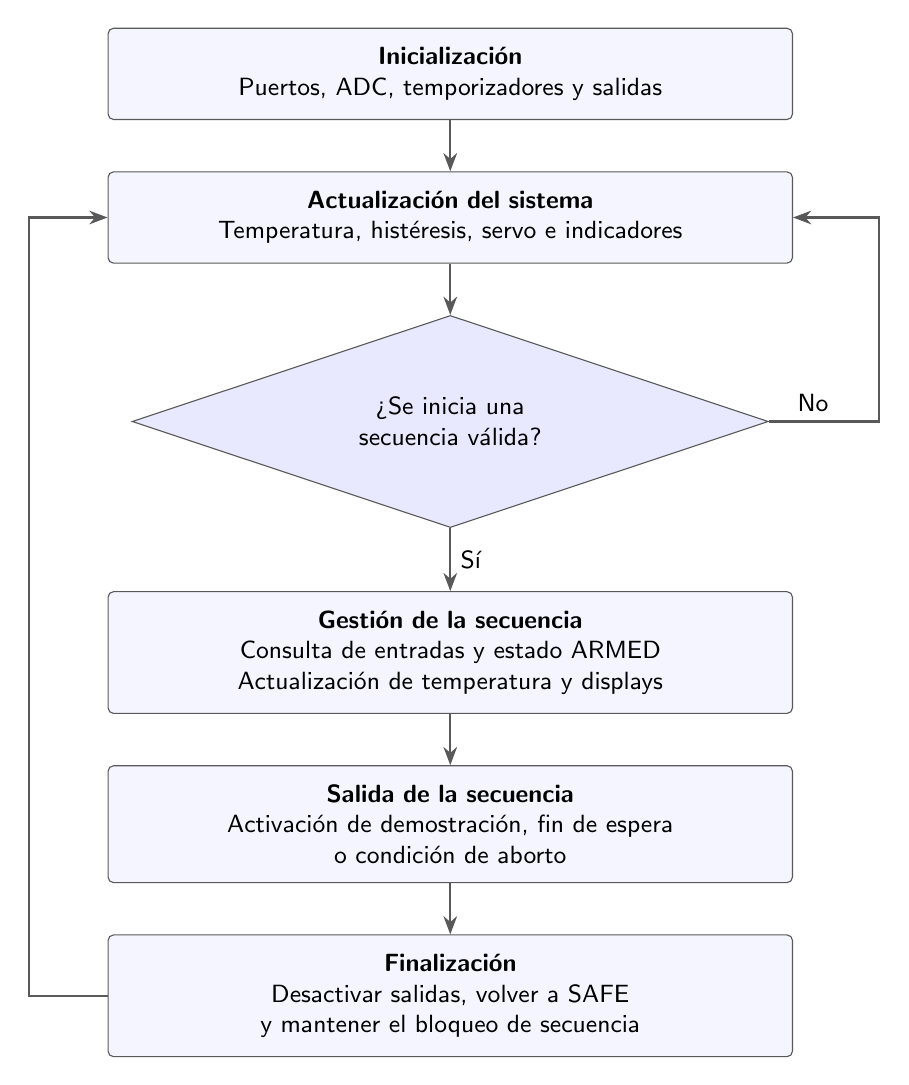
\begin{tikzpicture}[font=\sffamily\small,>=Stealth,
 caja/.style={draw=black!65,rounded corners=2pt,fill=blue!4,text width=8.2cm,align=center,minimum height=1.05cm,inner sep=7pt},
 decision/.style={diamond,draw=black!65,fill=blue!9,aspect=3,text width=5.7cm,align=center,inner sep=2pt},
 flecha/.style={->,thick,draw=black!65}]
\node[caja] (inicio) {\textbf{Inicialización}\\Puertos, ADC, temporizadores y salidas};
\node[caja,below=0.65cm of inicio] (medida) {\textbf{Actualización del sistema}\\Temperatura, histéresis, servo e indicadores};
\node[decision,below=0.65cm of medida] (valida) {¿Se inicia una\\secuencia válida?};
\node[caja,below=0.8cm of valida] (gestion) {\textbf{Gestión de la secuencia}\\Consulta de entradas y estado ARMED\\Actualización de temperatura y displays};
\node[caja,below=0.65cm of gestion] (salida) {\textbf{Salida de la secuencia}\\Activación de demostración, fin de espera\\o condición de aborto};
\node[caja,below=0.65cm of salida] (fin) {\textbf{Finalización}\\Desactivar salidas, volver a SAFE\\y mantener el bloqueo de secuencia};
\draw[flecha] (inicio)--(medida);
\draw[flecha] (medida)--(valida);
\draw[flecha] (valida)--node[right]{Sí}(gestion);
\draw[flecha] (gestion)--(salida);
\draw[flecha] (salida)--(fin);
\draw[flecha] (valida.east)--++(1.4cm,0) node[above,pos=0.4]{No} |- (medida.east);
\draw[flecha] (fin.west)--++(-1cm,0) |- (medida.west);
\end{tikzpicture}
\end{document}
